\documentclass[letterpaper,10pt]{article}
\usepackage[left=1.2in,right=1.2in,top=1in,bottom=1in]{geometry}
\usepackage{epsfig,endnotes}

\usepackage{adjustbox}
\usepackage{algpseudocode}
\usepackage{algorithm}
\usepackage{amsfonts}
\usepackage{amsmath}
\usepackage{amssymb}
\usepackage{array}
\usepackage[english]{babel}
\usepackage{balance}  % for  \balance command ON LAST PAGE  (only there!)
\usepackage{booktabs}
\usepackage{caption}
\usepackage{color}
\usepackage{comment}
\usepackage{datetime}
\usepackage{paralist}
\usepackage{epigraph}
\usepackage{eurosym}
\usepackage{fancyvrb}
\usepackage{filemod}
\usepackage[draft,inline,nomargin,index]{fixme}
\usepackage{float}
\usepackage{flushend}
\usepackage[T1]{fontenc}
\usepackage{graphicx}
\usepackage{hyperref}
\usepackage{ifthen}
\usepackage[utf8x]{inputenc}
\usepackage{listings}
\usepackage{lmodern}
\usepackage{makeidx}
\usepackage{marginnote}
\usepackage{mathpartir}
\usepackage{mathptmx}
\usepackage{mathtools}
\usepackage{mfirstuc}
\usepackage{multicol}
\usepackage{multirow}
\usepackage{parcolumns}
\usepackage{paralist}
\usepackage{pifont}
\usepackage{stmaryrd}
\usepackage{subfig}
\usepackage{tcolorbox}
\usepackage{tikz}
\usepackage[colorinlistoftodos]{todonotes}
\usepackage{url}
\usepackage{verbatim}
\usepackage{xcolor}
\usepackage{xifthen}
\usepackage{xspace}

\graphicspath{{./images/}}
\DeclareGraphicsExtensions{.pdf}

\renewcommand\UrlFont{\color{blue}\rmfamily}

\begin{document}

%don't want date printed
\date{}

\title{\huge \underline{Survival Guide} \\
Graduate Student Board (GSB) \\
Computer Science, Purdue university \\
\vspace{\baselineskip}
\large Last modified: \filemodprintdate{\jobname}}

\maketitle

\section{Introduction}
This guide provides information about the department, Purdue, the Lafayette area, Indiana, and surrounding states. The information in this guide is not complete and not guaranteed to be correct. If you are not sure about something, do not be afraid to ask a fellow student or to e-mail the CS Graduate Student Board (\emph{gsb@cs.purdue.edu}). If you would like something added or changed in the Guide, please e-mail the GSB.

\textit{Disclaimer: This document is not intended to describe departmental and school policies and is not a publication of the Department of Computer Sciences nor the School of Science.}

\begin{figure}[h]
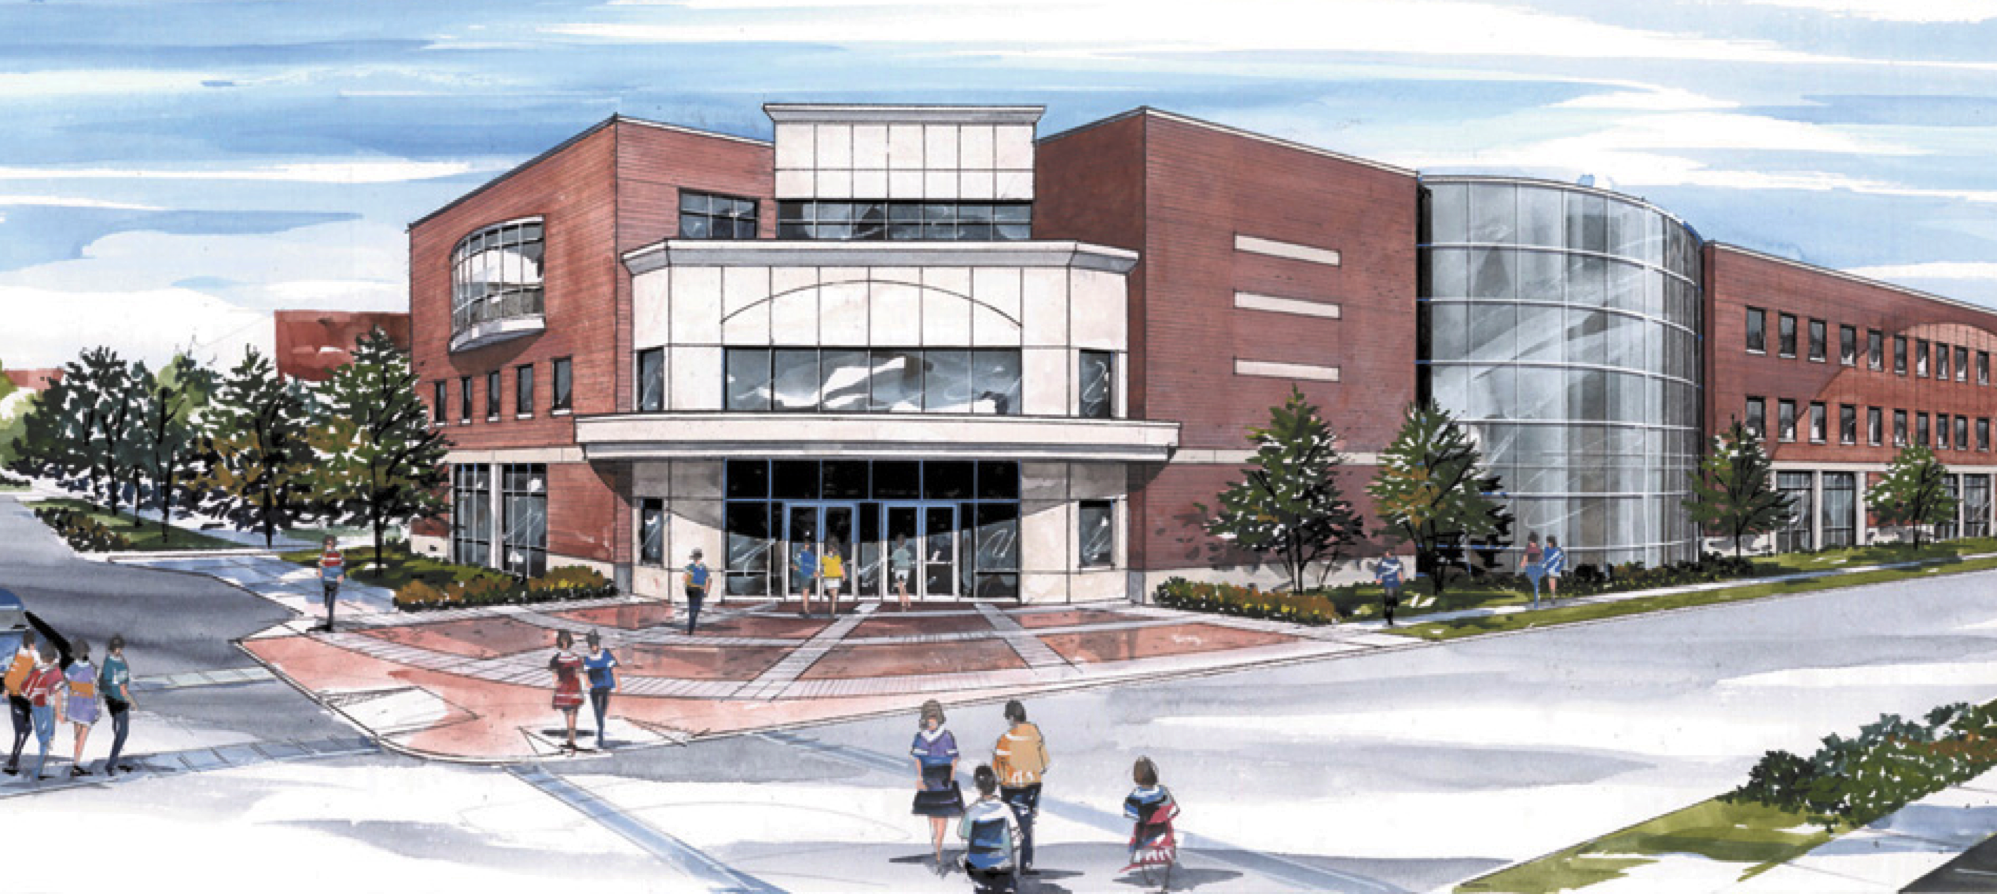
\includegraphics[width=1.0\textwidth]{lawson.png}
\end{figure}

\pagebreak
\tableofcontents

\pagebreak
\section{Acronyms}

During your first few weeks here at Purdue, you'll encounter many new acronyms and buzzwords. Here is a list of those used most frequently.

\begin{itemize}
	\item ACM --- Association for Computing Machinery. An international organization for computer scientists. Locally, ACM refers to the student ACM chapter which performs numerous services for the students.

	\item BO --- Business Office. This is the office that handles the money and some other matters related to the CS department. Located on the third floor.

	\item BOSO --- Business Office for Student Organizations. This is the office that handles the money and some other matters related to official student organizations. Hopefully, you will not have to deal with them unless you are an officer in a student organization in campus.

	\item CoRec --- Cordova Recreational Sports Center. This is one of Purdue's main sports facilities, where you can go practice a large number of sports and physical activities. In 1998 it was officially renamed the Recreational Sports Center, but many people still call it the Co-Rec.

	\item GSB --- Graduate Student Board. Represents the interests of graduate students in the department of computer science.

	\item ITaP --- Information Technology at Purdue. This is the university group that operates and maintains the main university computer system.

	\item PMU --- Purdue Memorial Union. The building next to Stewart Center.

	\item PAL --- Purdue Air Link. Purdue's wireless network.

	\item PUSH --- Purdue University Student Health center

\end{itemize}
\pagebreak
\section{Useful Links}

\begin{itemize}

	\item Off campus apartments --- \url{https://www.purdue.edu/offcampushousing}

	\item Boiler apartments --- \url{https://www.boilerapartments.com}

	\item Purdue Exponent --- \url{https://www.purdueexponent.org/classifieds}

	\item Parking --- \url{https://www.purdue.edu/parking}

	\item List of CS courses --- \url{http://www.cs.purdue.edu/academic-programs/courses}

	\item Register for the semester, pay fess, register for classes --- \url{https://mypurdue.purdue.edu}

	\item Blackboard --- \url{https://mycourses.purdue.edu}

	\item CS Profile --- \url{https://my.cs.purdue.edu}

	\item Research --- \url{https://www.cs.purdue.edu/research}

	\item Master's Curriculum --- \url{https://www.cs.purdue.edu/graduate/curriculum/masters.html}

	\item Ph.D. Curriculum --- \url{https://www.cs.purdue.edu/graduate/curriculum/doctoral.html}

	\item People --- \url{https://www.cs.purdue.edu/people/index.html}


\end{itemize}

\pagebreak
\section{For New Students}
\section{First Week on Campus}

This section presents, roughly, an outline of some of what you should do in your first week on campus.

\begin{itemize}
	\item Select courses (\url{http://www.cs.purdue.edu/academic-programs/courses/}) and register (\url{https://mypurdue.purdue.edu}). For late registration or for research credits, you need to ask your instructor/advisor to sign a Form-23 which you then need to take to the Registrar's Office (Hovde building).

	\item Get your student ID card: \url{http://www.purdue.edu/business/card/}

	\item Start a boiler express account (\url{https://dining.purdue.edu/}, look for eAccount) if you want, which you can use in dining courts cafes and other places on campus.

	\item Get a mailbox by asking someone in the mail room

	\item If you are an International Student, you should have gone through the orientation for International Students. If not, report to the ISS in Schleman Hall as soon as possible.

	\item Set up your profile in \url{https://www.cs.purdue.edu/people/graduate-students/index.html} which you can do via \url{https://my.cs.purdue.edu/}.

	\item Set up your personal webpage in your \$HOME/.www/ directory.

	\item Get a locker on Recreational Sports Center

\end{itemize}

Useful Links:
\begin{itemize}
	\item \url{http://www.cs.purdue.edu/academic-programs/courses/} --- List of CS courses

	\item \url{https://mypurdue.purdue.edu} --- Register for the semester, pay fess, register for classes

	\item \url{https://mycourses.purdue.edu} --- Blackboard, some instructors use this to upload course materials and for homework submissions

	\item \url{https://my.cs.purdue.edu/} --- CS Profile, e.g., classes taken, requirements fulfilled, advisor on record etc
\end{itemize}

\subsection{First Week on Campus}

This section presents, roughly, an outline of some of what you should do in your first week on campus.

\begin{itemize}
	\item Select courses (\url{http://www.cs.purdue.edu/academic-programs/courses/}) and register (\url{https://mypurdue.purdue.edu}). For late registration or for research credits, you need to ask your instructor/advisor to sign a Form-23 which you then need to take to the Registrar's Office (Hovde building).

	\item Get your student ID card: \url{http://www.purdue.edu/business/card/}

	\item Start a boiler express account (\url{https://dining.purdue.edu/}, look for eAccount or \url{http://www.purdue.edu/business/card/}) if you want, which you can use in dining courts cafes and other places on campus.

	\item Get a fob access key to the areas you are authorized to access by talking to Building Operations Coordinator (LWSN 1158).

	\item Get a mailbox by asking someone in the mail room.

	\item If you are an International Student, you should have gone through the orientation for International Students. If not, report to the ISS in Schleman Hall as soon as possible.

	\item Set up your profile in \url{https://www.cs.purdue.edu/people/graduate-students/index.html} which you can do via \url{https://my.cs.purdue.edu/}.

	\item Set up your personal webpage in your \$HOME/.www/ directory.

	\item Get a locker on Recreational Sports Center.

\end{itemize}


\section{Housing}

If you do not have any housing by the first week of the semester, run, do not walk, to the Dean of Students Office in Schleman Hall to obtain the Off Campus Housing listing and advice on obtaining a place to live. This information can also be accessed online via:

\centerline{\url{https://www.purdue.edu/offcampushousing}}
\vspace{\baselineskip}

Also check the Exponent:

\centerline{\url{https://www.purdueexponent.org/classifieds}}
\vspace{\baselineskip}

and Boiler apartments:

\centerline{\url{https://www.boilerapartments.com/}}
\vspace{\baselineskip}

for housing ads and roommate classifieds.
\vspace{\baselineskip}

Grad students often live in one of the Grad Houses or in Purdue Village. If you wish to live in Purdue Village (PV), you should apply ASAP. Purdue Village, which used to be only for married students, does allow single students. Spots in PV tend to fill up fast.

There are a numerous student apartment complexes all around campus and many old houses that have been divided into multiple living units. The apartments right around campus tend to be leased in January and February for the following fall semester, so start your search early in the spring for your fall housing. In addition, if you have a group of friends that you can live with, you can usually find an older house for rent if you check the classifieds. One other resource available to grad students is the Purdue Research Foundation (PRF), which has many old houses around campus for rent. Unfortunately for undergrads, PRF will only rent to faculty and grad students.

Apartments within walking distance of campus tend to be quite expensive but if you have transportation, there are numerous apartment complexes all over the Lafayette area that are quite reasonable. If you don't have a car, you can see if the bus line runs nearby. Of course, you always run a risk if you depend heavily on the buses. One more thing to consider when deciding on off-campus housing is related to restrictions on obtaining parking permits. The University will not sell you a parking permit if you live too close to campus. If you plan on driving to campus, make sure you live far enough away to get a university parking permit.


\subsection{Utilities}

If you are moving into an apartment or house, you will probably need to hook up some utilities. When you sign a lease, check with the landlord to see what utilities are not included in the rent. Then a few days before you move in to your new domicile, call the utility companies to hook up the necessary utilities. Many of the utility companies will demand a deposit for new service if you did not have an account with them previously. Examples of \emph{some} carriers are shown in the table below:

\begin{table}[h]
	\centering
	\begin{tabular}{@{}lll@{}}
		\toprule
		\textbf{Utility} & \textbf{Company} & \textbf{Phone} \\
		\midrule
		Cable & Insight Communications & 765-447-6886 \\
		Electric & Cinergy/PSI & 800-521-2232 \\
		Gas & Indiana Gas Company & 800-666-3090 \\
		Telephone & Verizon & 800-483-4600 \\
		Water & West Lafayette Water Company & 765-463-5531 \\
		Water & Lafayette Municipal Water System & 765-742-8404 \\
		\bottomrule
	\end{tabular}
\end{table}


The city of West Lafayette provides curb-side service for recycling and garbage pickup only for houses with four units or less. If you live in a complex or house with more than four units then a private contractor must be hired for garbage disposal. Labeled bins are provided for anyone wishing to drop-off recyclable materials at 705 S. River Road. There are also bins for recyclable materials around Purdue Village.
\section{Parking}

\begin{tcolorbox}[colback=green!5!white,colframe=green!75!black]
	\textbf{Note!} Purdue is increasing its efforts towards a greener campus. If you don't already own a car, consider alternative means of transportation. \textbf{CityBus} offers \textbf{fare-free} access to the CityBus system with a valid Purdue ID. In 2018, state street has been renovated to be more \textbf{bike} friendly.

	\vspace{\baselineskip}
	In addition consider these parking options:
	\begin{itemize}
		\item Low Emission Parking
		\item Charging stations for electric vehicles
		\item Use a Zipcar
	\end{itemize}
\end{tcolorbox}

Parking at Purdue can be a nightmare. Public parking near campus is in very short supply, and permit parking isn't much better. The largest public parking lot is behind the Stadium, quite a hike from the CS building. A, B, and C parking permits allow you to park on campus. A and B parking permits are for faculty and three-quarter time staff only, so students are normally limited to C parking permits.

\centerline{\url{https://www.purdue.edu/parking/}}
\vspace{\baselineskip}

A C parking permit allows you to park in C parking places, which are marked by red signs. Unfortunately, the C parking places are generally not close to the CS building with most of the C parking in a lot off State Street by the dorms, and near CoRec. To obtain a C parking permit, you must prove that you live more than 1.5 miles from campus (what they call walking distance). C Garage permits are also available. These allow you to park at the top of a specific parking garage.

If you drive but don't buy a permit, there is public street parking near the building on some of the side streets. However, these spaces are generally all gone by 8:30 am daily and most have a 3 hour time limit, for two reasons:

Many folks forget about this time limit, and their vehicles become easy prey for West Lafayette police who roam about with ticket pads armed and ready. The pointless shuffling of vehicles from one parking spot to another amuses the neighborhood children. Note that cars are time-stamped with a swatch of chalk on one of the rear tires so that the time they've been parked in one spot is known, and, therefore, the time that they're eligible for ticketing is known. Parking at night is no problem. All A, B, and C spots are open after 5 pm and on weekends. Also, never park in a 24 hour reserved spot; you will be ticketed and towed.

Residence hall parking permits are available to people living in Grad Houses or the Dorms. Stop by the Grad House or Dorm main office to inquire about permits, and check early since the number of residence hall permits is limited. One final note for students living in Purdue Village, you should stop by the PV office on Nimitz Drive after obtaining your Purdue permit in order to get a PV permit. It's free and allows you to park your car near your apartment.


\pagebreak
\section{Computer Science Department}
\section{History}

\begin{tcolorbox}[colback=green!5!white,colframe=green!75!black]
	Purdue Computer Science Department is the oldest CS department in the United States!
\end{tcolorbox}

In case you didn't know, Purdue's CS department is the oldest in the country, formally authorized in October 1962. Dr. Sam Conte was the first department head, serving until July 1979, when Dr. Peter Denning took over. Dr. Denning took a position with NASA in June, 1983 at which point Dr. John Rice became department head. After 13 years of distinguished service, Dr. Rice stepped down and returned to teaching. He was succeeded by Dr. Ahmed Sameh who came aboard during the 1996-1997 academic school year. Dr. Susanne Hambrusch, was appointed in the year 2002 and held the position until the summer of 2007. At that point in time Aditya Mathur took over as department head. In June 2012, Dr. Sunil Prabhakar has been appointed Head of the Department of Computer Science after a period of serving as an interim department head.

We are also one of the largest and most highly-rated departments in the country. We received more than 4,000 undergraduate applications for Fall 2017. Currently, 1,708 students are enrolled in the undergraduate program, an all-time high that more than doubles the number of students enrolled just five years ago.

The CS department was originally located in the Math building. In 1985, the CS department moved into a building all to itself. This building was formerly the Memorial Gymnasium. (The Memorial is to a group of Purdue students and alumni who died in a train wreck while traveling to a game). It has been completely renovated to hold us. During the renovation it was rumored that a swimming pool would be left in the basement, but this idea was apparently dropped. Finally, in the fall of 2006, the department moved into our new location, the Lawson Computer Science Building.

\section{Organizations}

\subsection{ITaP}
ITaP (Information Technology at Purdue) serves the entire university community (excluding administration). This includes Krannert (business school), Computer Sciences, and other divisions of the University. ITaP provides many varieties of computer systems, and administers several public computer labs and computing clusters.

For more in-depth information, check the schedule of ITaP short courses. These courses are taught by ITaP staff members. Usually they are given in the evening to avoid conflicts with classes or other activities. These courses give you a chance to ask specific questions and increase your knowledge about certain topics. Schedules appear in the ITaP Newsletter and are posted on various bulletin boards. For more information about courses, please visit \url{https://training.purdue.edu}



\subsection{GSB}
The Computer Science Graduate Student Board is the liaison between the department administration and its graduate students. The Graduate Student Board is also affiliated with the Purdue Graduate Student Government. GSB organizes technical talks, pizza parties, summer picnics, bowling nights, movie nights, participates in the graduate and undergraduate committees, and the faculty search process. To learn more about the Graduate Student Board, visit \url{https://www.cs.purdue.edu/gsb/}.



\subsection{ACM}
The International Association for Computing Machinery is an international professional and educational organization dedicated to advancing the art, science, engineering, and application of information technology. The local chapter is open to all Purdue students interested in the field of Computer Science. The goal of the local student chapter is to aid and support student academic, professional, and social development.

ACM supports a number of developmental activities as well as social events throughout the year. ACM sponsors the orientation program for graduate students, the Computer Science fall picnic, programming contests, monthly pizza parties, and guest lecturers. ACM also compiles and distributes the Computer Science Resume Book.

Early in the fall semester, ACM invites Computer Science students to submit resumes which are compiled into a book. The Resume Book is distributed to any company willing to donate a nominal sum. Last year over 100 students participated and over 60 companies donated. The Resume Book sale is ACM's main fund raiser and a great way for students to distribute their resumes to potential employers.

To learn more a bout Purdue ACM visit \url{https://acm.cs.purdue.edu/}.



\subsection{CSWN}
The Computer Science Women's Network (CSWN) is an organization at Purdue University consisting of people (both students and staff) who are dedicated to helping women in the field of computer science. The leadership team that organizes most activities is made up of female students who want to reach out and help all of the women in CS.

CSWN organizes different activities meant to encourage young women to meet one another and also learn more about their chosen field of study. These activities range from picnics to technical talks to helping students find tutors if they are needed. Their goal is to encourage women in computer science to stay in the field and prosper. For information, visit CSWN web site \url{https://www.cs.purdue.edu/cswn/}.



\subsection{USB}
The undergraduate student board is the liaison between undergraduate students and the department administration. For more information, visit \url{https://www.cs.purdue.edu/usb/}.






\section{Books}

There are a number of bookstores around campus that will be happy to take your life savings in exchange for a text book. University Book Store's main location is across the street from the Union at 360 W. State Street. University Bookstore is the original home of Purdue Pete. The Book Store used Purdue Pete for their logo, and the University later adopted him as the Purdue Mascot. University Book Store also has a smaller branch across from Mackey Arena at 720 Northwestern Avenue. Follett's Bookstore has two locations, 1400 W. State Street in Purdue West and 714 Northwestern Avenue across from Lambert Fieldhouse.

\begin{table}[h]
	\centering
	\begin{tabular}{@{}lll@{}}
		\toprule
		\textbf{Name} & \textbf{Location} & \textbf{Phone} \\
		\midrule
		Follett's Bookstore & Purdue West & 765-743-9642 \\
		Follett's Bookstore & Northwestern Ave & 765-743-9696 \\
		University Book Store & State Street & 765-743-9618 \\
		University Book Store & Northwestern Ave & 765-743-9432 \\
		\bottomrule
	\end{tabular}
\end{table}

Text books are sometimes held on reserve in the Undergraduate Library or the Math Library. A few CS text books are also available in the Undergraduate Student Office and the Graduate Student Office in Lawson.



\pagebreak
\section{Academics}
\section{Research}

Part of the reason that the department is highly-regarded is that the faculty are active in research, publications, and service to the CS community. It would take pages to describe all the current research projects. Therefore, for reference, the department Research page and Annual Reports page contain a summary of current projects:

\centerline{\url{https://www.cs.purdue.edu/research/}}
\vspace{\baselineskip}
\centerline{\url{https://www.cs.purdue.edu/about/annual_reports.html}}
\vspace{\baselineskip}

There is a research project for anyone here. There are research centers and institutes specializing in particular topics, a complete list of which is given at:

\centerline{\url{https://www.cs.purdue.edu/research/centers.html}}
\vspace{\baselineskip}

Most notably, the Center for Education and Research in Information Assurance and Security (CERIAS) is currently viewed as one of the world's leading centers for research and education in areas of information security that are crucial to the protection of critical computing and communication infrastructure. CERIAS is unique among such national centers in its multidisciplinary approach to the problems, ranging from purely technical issues (e.g., intrusion detection, network security, etc) to ethical, legal, educational, communicational, linguistic, and economic issues, and the subtle interactions and dependencies among them. CERIAS evolved from the COAST (Computer Operations, Audit, and Security Technologies) lab in 1999, which was a multiple project computer security research laboratory in Purdue's computer science department. For more information please refer to \url{https://www.cerias.purdue.edu}.

In addition, there are a number of groups that offer research seminars on a weekly basis:

\centerline{\url{https://www.cs.purdue.edu/research/seminars.html}}
\vspace{\baselineskip}
\section{Courses}

First, look at the list of courses being offered on the CS Department web site:

\centerline{\url{https://www.cs.purdue.edu/academic-programs/courses}}
\vspace{\baselineskip}

If you are a first-year Master's students, you will face many choices of classes. The choices for a first-year Ph.D. student are somewhat restricted. Talk to second or third year graduate students. The best place to get information about a course and a professor is from someone who has taken the course, and not necessarily your advisor or professors in the department. This is probably the most important step in the registration process.

Most people find it best to select courses so that their workload is balanced among various types of work: reading, programming, theory, mathematics (calculus, real analysis, linear algebra), etc. Taking two heavy programming courses together is a lot of work, three can be suicidal.

There is also the number of course hours to consider. Typical and maximum course loads are shown below. Keep in mind that what is said to be "typical" below may be a lighter or heavier load than what is right for you. If you are a Master's candidate, how much of a rush you are in to complete your degree will also be a factor. Taking the maximum number of credit hours in your first semester, however, is probably a recipe for disaster.

Credit Hours:
\begin{itemize}
	\item fellowship or self-supported 9 - 12 hours typical, 18 hours maximum
	\item quarter-time assistantship 6 - 12 hours typical, 15 hours maximum
	\item half-time assistantship (most TAs) 6 - 9 hours typical, 12 hours maximum
	\item half-time research assistantship (most RAs) less than 18 hours, at least 6 hours thesis work
	\item full-time research assistantship less than 18 hours, at least 12 hours thesis work
\end{itemize}

You can find the requirements for a Master's and Ph.D. students here:

\centerline{\url{https://www.cs.purdue.edu/graduate/curriculum/masters.html}}
\vspace{\baselineskip}

\centerline{\url{https://www.cs.purdue.edu/graduate/curriculum/doctoral.html}}
\vspace{\baselineskip}

A graduate student is classified as a full-time student if he or she is registered for 6 credit hours when funded by an assistantship or 9 credit hours when funded by a fellowship. Master's students need (eventually) to complete 10 three-credit courses, or 8 three-credit courses with a thesis, for their degrees. One of CS 502 or CS 565, one of CS 503 or CS 536, and CS 580 are required; the others are chosen by the student. You should get an idea of the courses you might like to take now, but don't bother trying to work out a schedule more than a semester in advance --- the actual scheduling of courses (regardless of what the course descriptions say) is quite variable. There are also "topics" courses that are offered each semester, some of which you might find interesting. A 590 topics course is directed study for students who wish to undertake individual reading and study on approved topics. A general topics course is worth three credit hours. It usually takes three to four semesters to complete the work for a Masters degree.



\section{Courses Descriptions}

This section contains descriptions of CS courses that are offered on the graduate level in our department. It does not include courses offered by other departments (i.e. MATH, EE, STAT, MGMT) that are also available to obtain graduate credit in the M.S. and Ph.D. programs in CS. For transferring credit check with your academic advisor, or with Secretary to the Graduate Office:

\centerline{\url{https://www.cs.purdue.edu/people/staff/index.html}}
\vspace{\baselineskip}

As there are substantial differences among the courses offered in regard to the amount and type of work for assignments, projects, in-class presentations, term papers, and exams, we are presenting a table that shows the major differences among these courses. The info given is mostly drawn from an old survey among graduate students in our department in Spring 1993, although some additions have been made for courses which were not included in the 1993 survey. Although some of the courses have changed over the years, this list will give you a rough idea of the type of workload to expect. However, course contents and workload depend considerably on the professor who teaches the course. The same number of programming assignments for two courses does not necessarily indicate a comparable effort in writing the code. Therefore, nothing presented here should be taken literally, only as an outline. Do not be afraid to talk to the professor who will teach the course and ask him more detailed information. Note that not all courses are offered every semester. Furthermore, it is not our purpose to show you a way to a degree at Purdue with the least possible effort, but to give you the chance to balance your course load for each semester according to your interests and degree program requirements.

The official prerequisites listed on the course pages are not completely accurate in terms of what you really need to succeed in a course. The survey disclosed that unstated prerequisites for nearly every course. It is not absolutely necessary to know these to do well in every course, but knowing them can greatly increase your efficiency. A comment nearly everyone made at some point was: ``Course are hard and require lots of work ... but in the end it's worth it.'' So, you can look forward to a lot of pain during the semester, and a very good feeling afterwards.

\begin{table}[h]
	\centering
	\begin{tabular}{@{}lp{5cm}p{9cm}@{}}
		\toprule
		\textbf{Course} & \textbf{Course Name} & \textbf{Load} \\
		\midrule
		CS 502 & Compiler Design & written(1), program.(5), proj.(1), quizzes(1), midterm, final - heavy programming \\
		CS 503 & Operating Systems & written(1), program.(5), proj.(1), midterm, final - heavy reading, heavy programming \\
		CS 510 & Software Metrics & - moderate reading \\
		CS 514 & Numerical Analysis & written + program.(8), midterm, final - math and programming \\
		CS 515 & Analysis of Linear Systems & - math \\
		CS 520 & Computational Methods & written + program.(10), proj.(2), midterm, final - math, problem solving, big projects \\
		CS 525 & Parallel Computing & written, program, midterm, final \\
		CS 526 & Information Security & written(5), project(3), midterm, final \\
		CS 530 & Intro. To Scientific Visualization & written, program, midterm, final \\
		CS 535 & Computer Graphics & program.(4), midterm - very heavy programming \\
		CS 536 & Computer Networks & written(5), program.(3),midterm, final - reading, heavy programming \\
		CS 541 & Database Systems & written(5), program.(2), midterm, final - reading, light programming \\
		CS 542 & Distributed Database Systems & written(3), proj.(1), midterm, final - reading, light programming \\
		CS 543 & Simulation and Modeling & written(2), program.(6), proj.(1), presentation(1), midterm, final - heavy programming \\
		CS 555 & Cryptography & written(6), proj.(1), midterm, final - moderate reading and problem solving, math \\
		CS 565 & Programming Languages & written + program.(5), proj.(2), midterm, final - heavy reading, theory, projects \\
		CS 580 & Algorithm Design & written(8), midterm, final - theory and problem solving \\
		CS 584 & Theory of Computation & written(10), presentation(1), quizzes(2), midterm, final - theory, participation in class \\
		CS 603 & Advanced Operating Systems & - reading, systems programming \\
		CS 614 & Ordinary Differential Equations & - math \\
		CS 615 & Partial Differential Equations & - math and programming \\
		CS 636 & Internetworking & program.(3), proj.(1), presentation(2), quizzes(2), oral final - heavy programming, participation in class \\
		\bottomrule
	\end{tabular}
\end{table}



\subsection{Registering}

You can register for courses by visiting \url{https://mypurdue.purdue.edu}, under the registration tab. Select the School term you need and if required enter the Registration PIN Verification, which is usually "999999".

For late registration or for courses that require the instructor's permission you need to fill a course-request form (Form-23), which you can get from the CS Graduate Office (LWSN 1137). After completing the form and have your instructor/advisor sign it, you need to take it to the Registrar's Office in the lowest level of Hovde Hall, Room 45.

You should be able to verify your registered classes through \url{https://mypurdue.purdue.edu}.
\section{Colloquia}

Some of the biggest names in computing will visit Purdue while you are here. Some of the visitors are big-names-to-be. When they visit, you want to attend these talks. Some will be boring, some will be incomprehensible, but they will give you a view of computing and current research that you probably can't get any other way. You might even get an idea for a research topic from the talk.

The current faculty sometimes give talks, including CS590 and CS690 seminars. Again, this is a good way to get exposure to some interesting research and faculty here at Purdue. Although you may wonder about it sometimes, the CS faculty here at Purdue is one of the best in the country. Take advantage of your time here to hear what they think is interesting.

If a faculty search is on for the year, there will be lots of faculty candidate talks in the spring semester. Attendance at these talks is beneficial both to you and the department. The department takes into consideration feedback from students when making a hiring decision, so please attend these talks and give your feedback to a GSB representative after candidate-student meetings which will be announced at least a week in advance.
\section{Ph.D.}

The basic requirements for getting a Ph.D. at Purdue are fairly straightforward, as described here: \url{https://www.cs.purdue.edu/graduate/curriculum/doctoral.html}. This section focuses on giving some advise beyond these basic requirements.

\subsection{Advisor}
Your advisor will be the person overseeing your research while you work on your dissertation. In other words, a thesis advisor is a combination of a friend, co-worker, guru, and mentor figure. He or she will therefore be one of the more important people in your life for the next few of years, so choose carefully. Desirable traits in an advisor include:

\begin{itemize}
	\item Easy for you to get along with
	\item Interested in the same area(s) you are
	\item Will not be leaving in the next couple of years (that you can tell)
	\item Can supervise your work closely (if you like that)
	\item Won't pressure you (if you want it that way)
	\item (Optional) Has grant money to support you
\end{itemize}

Usually, you talk to several professors in your area before making a decision. It is possible to change advisors after making your decision, but it is not generally recommended because it tends to delay your graduation.

\subsection{Plan of Study}
Once you have an advisor, your next job is to form the rest of your advisory committee. These will be the people who read your thesis, point out flaws, and eventually decide whether you have done Ph.D.-caliber work. Therefore, they are important people in your education. You and your advisor find (at least) two other professors interested in your area to be on this committee, one of which should be a senior faculty member. About the time you are doing this, you should also file a Plan of Study, an official document telling the administration what classes you have taken, what courses you plan to take, your area of interest, and other vital information. This can be done via \url{https://mypurdue.purdue.edu}.

\subsection{Thesis}
Now that you've demonstrated your aptitude at passing hard tests, and thus qualified yourself for research work, you have to thrash about, reading landmark papers from your area, trying to find a thesis topic. Remember that your goal at this point is to find a topic that you can learn to do research on; that's what the degree process is about. The topic doesn't have to be earth-shattering; in fact, you'll probably get out much more quickly if it isn't. Save the good stuff for when you're on your own trying to get grants and such. Also, consider that by the time you get done with your thesis, you will be eating, sleeping, living and breathing your topic. Try to pick something that you can survive becoming incredibly intimate with for 12 to 24 months; also, by the time you're done, you'll probably be burned out on the topic, so pick something you won't regret not working on for some time after you've graduated.

Once you've figured out exactly what it is that you're going to research, take your Preliminary Examination (usually known as Prelims). The party line on this exam is that it tests the student's competence in a research area and readiness for research on some specific problem. In practice, it is a public thesis proposal, given so that your committee can see what you've been up to, where you're headed, and give constructive criticism. The Graduate Committee will appoint one extra member to your advisory committee for this exam, presumably to keep everyone honest. Usually, this exam is given after you get your first results (publication) on your thesis topic.

Now, work like crazy, trying to prove whatever it is that you're trying to prove. Build, measure, tear down, read, build some more, and conclude. Write it all down in a nice form; we'll call that your \emph{dissertation}. Hope no one else is doing exactly the same thing at another university; if they are, and manage to publish their results before you, even by one week, you're probably out of luck, and have to start all over again on a new topic. Get your committee to agree that they like your dissertation. Then you have to make it satisfy the department's rules for Thesis Format, which define what a CS dissertation must look like, dealing with margins, figures, captions, etc.

Finally, schedule a final defense. This is a public oral exam before your committee and anyone else that cares to come; it is where you present what you've done for the past few years. It's also the last chance for people to pick your work apart and point out flaws. Hopefully, your committee will have pointed them out before the defense, so you have all the answers right at your fingertips. If you've done all your work, this should be a breeze.


\section{Funding}

Most people are funded by either a Teaching Assistantship (TA), a Research Assistantship (RA), or a Fellowship. Some people have sources of funding outside of these three types, but it is uncommon. To be considered a "full-time" student, you must register a certain amount of hours depending on your type of funding. TAs and RAs need to have 6 credit hours, while Fellows need 9. Being considered a full-time student has many benefits that include your ability to receive student health insurance, government loans, etc.

Most students enter the department with a Teaching Assistantship. If you are going to be a teaching assistant, you are probably wondering just what your duties will be. Your teaching assignment will probably fit into one of the following three categories:

\begin{itemize}
	\item A recitation instructor teaches recitation sections which normally consist of 20-30 students. The class will also have other lecture sections that are taught by the professor in charge of the course.
	\item A lab instructor teaches lab sections which normally consist of 15-25 students. The class will also have other lecture sections that are taught by the professor in charge of the course.
	\item A grader grades assignments, projects, and possibly exams for a course that is taught by a professor or another TA.
\end{itemize}

It is very rare that a teaching assistant is the sole instructor for a course, but it has happened in the past, for senior Ph.D. students. Teaching assignments are often not finalized until the week before classes begin. If you did not receive your teaching assignment before arriving at Purdue, talk to the graduate office. Once you have learned your assignment, contact the supervisor of the course as soon as possible. Also, all new teaching assistants must attend ``training sessions'' during the week before classes. These sessions will explain nearly everything you need to know about being a TA.

As a TA, you will be responsible for holding office hours, usually at least two hours a week. If your office hours schedule looks like a typical class schedule (e.g., MWF 1:30-2:30), you risk shutting out students who happen to have a class in that slot. It is much better to make your office hours schedule somewhat irregular. If you are financially supported by the department (TA, RA, grader) and need supplies for your work, they can be obtained in the mail room, LWSN 1151. The secretaries maintain a supply of paper, transparencies, manila folders, tape, pens, and pencils for instructors' and researchers' use.

Depending on your temperament, teaching can either be great fun or a terrible burden. On the positive side, you get paid for the work, you get to meet a lot of new people, and you get to see your students learning and share in their learning process. On the negative side, your students constantly pester you for information and answers, especially before an exam or the due date of a big project. Also, be assured that students will not confine requests for assistance to your office hours. If you have any problems with your assignment, see the course instructor or someone in the graduate office.

Research Assistantships are given to you by a professor who has procured funding from, typically, an outside source such as a government agency (e.g. NSF) or a corporation. Ideally, your RA will support work that interests you and work that will contribute toward your Master's or Ph.D. thesis.



\pagebreak
\section{Purdue University}
\subsection{About}

As the story goes, when other college teams met the Purdue football squad they were in awe of the size of the Purdue players. Believing that no man of academic ability could be so enormous, rivals were sure that the Purdue team was made up of workers from the old Lafayette Boiler Factory. Hence, Purdue was the victim of many insulting names, one of which was "Boilermakers".

Other tellers of this tale (probably Purdue opponents) state that the team members actually were boilermakers and not students. Do not believe them. Purdue, being a famous agricultural school, attracted many farm boys who were typically large, healthy, and powerful.

Many Boilermaker alumni have distinguished themselves in one way or another. A few of them are Neil Armstrong, Birch Bayh, Earl Butz, Eugene Cernan, Len Dawson, Bob Griese, Durwood Kirby, Chris Schenkel, Orville Reddenbacher, Roger Chaffee, Virgil Grissom, Abe Gibron, John Wooden, Hank Stram, and Herbert Brown.

Sports have always been big at Purdue, gaining the support of students and nearby residents alike. As a member of the Big Ten football league, Purdue went to the Rose Bowl in 1967 and beat Southern California 14-13. In 1978 the Boilermakers went to the Peach Bowl and beat Georgia Tech 41-21. In 1979 they went to the Astro-Bluebonnet Bowl and beat Tennessee 27-22. The 1980 Liberty Bowl saw Purdue squeak by Missouri, 28-25. Then Purdue suffered three straight losing seasons, before an impressive 1984 season, which ended in a 27-24 loss to Virginia in the Peach Bowl. The team then languished in obscurity until the arrival of coach Joe Tiller. Tiller's Boilermakers have now played–and won–the Alamo Bowl two years running, returning pride to the hearts of fans everywhere. As of 1999, the men's basketball team has shared six Big Ten championships in the last 16 seasons. Three of them came from 1994, 1995, and 1996! The 1987-88 season was the sixth straight year the team won 20 or more games and qualified for NCAA tournament action. Not to be left behind, the women's basketball team was national champion in 1998!

The “All-American” Marching Band is one of the largest university bands in the Big 10 and the nation with 320 members. Highlights of that band include the World's Largest Drum (Built in 1921) and the Golden Girl (A tradition since 1954). The Department of Bands also boasts two to four concert bands each semester and three jazz bands, as well as a 100-member symphony orchestra and the university's pep bands.

The present Purdue seal was adopted in 1974. The griffin head sits on a 3-sectioned shield which represents the 3 educational thrusts of Purdue: science, technology, and agriculture. The lines representing the griffin's mane are for the 5 campuses: West Lafayette, IUPU Fort Wayne, North Central, Calumet, and IUPU Indianapolis.

The Purdue Mascot is the Boilermaker Special V, the locomotive which can be seen around campus primarily before home football games.

Purdue is one of 68 land-grant colleges established with the Morrill Act, an act signed by President Abe Lincoln by which the federal government offered to turn over public lands to any state which would use the land to maintain a college for the study of agriculture and the mechanical arts. The Indiana General Assembly accepted $150,000 from John Purdue and $50,000 from Tippecanoe County. In 1874 classes began at Purdue University with 6 instructors and 39 students.

The West Lafayette campus, including housing areas, recreation areas, the airport, and service areas, covers 2,307 acres. Additional lands away from West Lafayette are used for agriculture and recreation.

The Edward C. Elliott Hall of Music (seating 6,077, it is considered the largest and best-equipped theater of any educational institution in the world), the Loeb Playhouse (seating 1,052), the Experimental Theater, the Memorial Union, Stewart Center, Slayter Center, Ross-Ade Stadium (capacity 67,861), and Mackey Arena (seats 14,123) make Purdue a cultural and recreational center for northwestern Indiana.

The Purdue Airport, established in 1930, was the first university-owned airport in the country.


\subsection{Buildings}

\subsubsection{Lawson Computer Science Building}
Where most faculty, students, and research labs are located. The administrative staff for the CS department is located here. The basement houses the TA offices and computer labs for students. The 3rd floor has a balcony that overlooks University St. and 3rd St.



\subsubsection{Felix Haas Hall}
The main computer science building until Lawson was completed in Fall 2006. Even though other departments have taken over much of the space, a few labs and faculty still remain in this building.



\subsubsection{Recitation Building}
Until a few years ago, the Recitation (REC) building, directly east of MATH, was only of interest if you had a class there. Starting from the Fall of 1999, however, the second floor of REC is home to the Center for Education and Research in Information Assurance and Security. CERIAS grew out of the COAST laboratory in Computer Science, but with its current Center status is able to have a much larger multidisciplinary reach, although it still has very strong connections with CS. Several CS faculty and staff members as well as grad students have offices there.



\subsubsection{Adminstrative Offices}
Schleman and Hovde Halls are the main student services and administration buildings. There are a number of major administrative attractions in these two buildings.

Hovde:
\begin{itemize}
	\item The Registrar's Office
	\item The Bursar's Office
\end{itemize}

Schleman:
\begin{itemize}
	\item The Dean of Students Office
	\item The Admissions Office
	\item Registration Headquarters
	\item International Student Services
	\item Business Office of Student Organizations
\end{itemize}



\subsubsection{Purdue Memorial Union}
The Memorial Union (in memory of Purdue alums killed in wars) was built back when it was stylish and economically feasible to incorporate a good deal of wood in finishing the interior of a building. The varnished woodwork, solid wood tables and chairs, and stone and wood floors are a refreshing change from the plastic, concrete, veneer and linoleum which surrounds you in most places. Also featured are lots of old moldy plaques commemorating people who would otherwise be forgotten, and a 3-D model of the campus (a must for visiting parents).

Functionally, the predominant features of the Union are eating places, meeting places (various ballrooms and lounges), and sleeping places (the “Union Club” hotel rooms for convention attendees, visiting parents, etc.). For details about the eating places, see the section about on-campus dining.



\subsubsection{Stewart Center}
From here it is possible to walk through tunnels and buildings all the way to either Grad House without going outside, as well as to either of the three parking garages, Marsteller Street (across from Hawkins Grad House), Wood Street (across from Young Grad House), or Grant Street (across from the Union). The main attractions of the Stewart Center are:

\begin{itemize}
	\item Fowler Hall, on the first floor, an auditorium equipped for movie screenings
	\item Loeb Playhouse, the Purdue Experimental Theatre
	\item An Art Gallery, off the west foyer on the first floor
	\item HSSE library, on the first floor, see the section on libraries for details
	\item An ITaP Lab, first floor, often very crowded
	\item ITaP Customer Service Center, on the ground floor, room G68, phone 49-44000; a first and single point of contact for support with many ITaP services
	\item Audio-Visual Center, ground floor
	\item Candy Stand, main floor, sells candy to rot your teeth, paperbacks to rot your mind, and practically every magazine you've ever heard of plus hundreds more that you've never heard of
	\item Envision Center, on the ground floor level between Steward Center and PMU
\end{itemize}


\subsubsection{International Student Services}
The Office of International Students and Scholars in located in Schleman Hall. ISS is a division of International Programs and offers many services that are useful to foreign students. ISS is the expert resource for the University in the areas of F-1, J-1, and H-1B rules and regulations. The office, SCHL 136, is open between 8:00 am and 5:00 pm each weekday, and if you are an international student, you will be visiting every now and then. They are nice folks, even though they may appear a bit harried when you first encounter them around orientation time. To learn more about ISS, visit \url{http://www.iss.purdue.edu}.



\subsubsection{PUSH}
The Purdue University Student Health Center (PUSH) is where the folks with white coats, stethoscopes, and benign smiles are simply waiting to have a look at your innards. They provide the health services to full and part-time students and their spouses, and in certain cases to Purdue employees and visitors.

The hours of operation below are for the regular semesters; while the appointment desk is stays on the same schedule during the summer, some other offices have somewhat reduced hours during summer session and between sessions.

The following services are available without charge. Many of the doctors will accept appointments and a walk-in service is always provided during clinic hours. Walk-ins are first-come-first-serve and you should expect a 15 to 40 minute wait.





\subsection{Food}


\subsubsection{Campus Food}
If you live in one of the dorms or one of the grad houses, you have a cafeteria available for all your eating needs. The Lawson Computer Science Building, The Purdue Memorial Union, and Stone Hall also have cafeterias which are available to the general public.

The Port - Located in the Lawson Building. You immediately see it when you enter the front door. Breakfast items, fruit, sandwiches, mini-pizzas, soup, salad, coffee, and smoothies can be found here.

Purdue Memorial Union - The Union offers a wide range of food for breakfast, lunch, and dinner at reasonable prices. There is a cafeteria with a variety of cafeteria foods. Purdue students are tax exempt at the cafeteria, so be sure to bring along your Student ID. The Union also serves pizza, ice cream, burgers, and other munchies on the ground floor.

Restaurants surround the campus on every side. Some of the more popular eating establishments are located in Purdue West, The Village and Chauncey Hill Mall, and the area north-east of campus.


\subsubsection{Produce}
In the fall, you can buy one-gallon jugs of apple cider and ten-pound bags of apples (many varieties) at the Purdue Farm. Prices are comparable to those in local grocery stores, but the quality is much higher. Sometimes they also sell pumpkins, squash, and other fall vegetables. The farm is located about 3 miles west on State Road 26 from the Purdue West Shopping Plaza. Watch carefully for signs on the left. Turn off (left) after passing the orchard. The farm is about 1/4 mile on the right.



\subsubsection{University Meat Market}
Purdue offers classes in butchery, and where there's a butcher, there's raw meat. The fruits of the aspiring butchers' labors are sold each Wednesday from 3:00 to 5:30pm and Friday from 12:00 am to 4:30 pm in Smith Hall, room 170. (Smith Hall is on the south side of State St., nearly due south of Matthews Hall. Room 170 is in the west wing of the building.) Most of the common cuts of beef and pork are produced, though not all cuts are available every week. Occasionally, turkey and lamb are also available. As with produce, the prices are comparable to those in local supermarkets, but the quality is outstanding (which is what you will be if you don't get there early and beat the rush). If you need more information about the Boilermaker Butcher Block, call them at 49-48285.






\subsection{Events}


\subsubsection{Concerts and Convocations}
The Department of Convocations sponsors a wide variety of events including:

\begin{itemize}
	\item chamber music groups
	\item individual virtuoso musicians
	\item various symphony orchestras and ballet troupes
	\item theatrical companies doing musical plays and revues
	\item individual performers
\end{itemize}

Many of the events have ``big names,'' and most are worthwhile.

Near the beginning of fall semester, slick brochures appear around campus describing the coming year's slate of convocations and the season ticket options available (these are usually cheaper; amounting to getting one or two of the tickets free when compared to the single ticket price). If you are buying season tickets, you must decide upon the series you want to buy (there are several and they sometimes change over time) or commit to a number of performances of your own choice. The brochures describing the coming events state which series contains which convocations. Also, several weeks before each event, ads appear in the Exponent (campus newspaper) stating when individual tickets will be sold.

With a student ID, you can buy Convocations tickets at the (lower) student rate. This also applies to season tickets. For further information, go to \url{https://www.purdue.edu/convocations/} or to the ticket office at the north end of the lobby in the Hall of Music or to the ticket windows in Stewart Center, located at the south end of the lobby with the mural.




\subsubsection{Sports}
Purdue is part of the Big 10 conference and people around here go crazy for football and basketball. However, non-revenue sports events at Purdue are rather poorly attended. University fees include an activity fee which entitles students to reduced tickets for sporting events such as football, basketball, and volleyball.

With a student ID, you get reduced price season football tickets. Single game tickets are also available, but in most cases they cannot be purchased at discounted price.



\subsubsection{Movies}
The Purdue Student Union Board (PSUB) regularly schedules film series each semester. The movies are shown on Friday and Saturday evenings in Fowler Hall which is part of the Stewart Center. Show times are usually at 7:00 and 9:30 PM. For PSUB calendar of events, see \url{https://union.purdue.edu/studentevents/}.




\pagebreak
\section{Lafayette}

\subsection{General Description}
The greater Lafayette area has a population of over 85,000, with approximately one-third of that number residing on this side of the river. This population increases about 30 percent when Purdue is in session. The Wabash River separates the cities of West Lafayette and Lafayette. West Lafayette and Lafayette are two distinct cities connected by a number of bridges. If a resident hears you say that West Lafayette is a part of Lafayette or that Purdue is in Lafayette you should immediately fear for your well-being. Remember, Purdue is in West Lafayette.

Lafayette was founded in 1825 by William Digby who named the town after French General Marquis de Lafayette on Lafayette's visit to America that year. Lafayette became a thriving commercial center because of its location on the Wabash River and its proximity to the Old Wabash and Erie Canal. West Lafayette was created in 1866 with the name of Chauncey when the town of Chauncey merged with the town north of it, Kingston. Plans for Purdue were set in 1869 and classes began in 1874. In 1888, Chauncey was renamed West Lafayette.

Purdue is the largest employer in Tippecanoe County. (Tippecanoe is an Indian name for buffalo fish.) Many other industries have been attracted to this area including Alcoa Aluminum, Duncan Electric, Eli Lilly Pharmaceuticals, Fairfield Manufacturing, Landis \& Gyr, National Homes, Ralston Purina, Great Lakes Chemical, Subaru-Isuzu, and Caterpillar Tractor.




\subsection{Weather}
The weather in Lafayette is a constant source of conversation. Summers tend to be hot and winters tend to be cold but the weather is never predictable. One day you may be wearing shorts, and the next day you may be bundled in your warmest winter clothes. Most winters include snow with heavy snowfall at times. The wind-chill factor will occasionally drive the temperature down to or below (Celsius or Fahrenheit, at it really doesn't matter). Spring weather is windy with wide temperature ranges. Some days are very pleasant and others very rainy. Summers bring big thunderstorms and high humidity. Indiana has one of the highest tornado-hit rates in the nation, and Tippecanoe County enjoys the distinction of having the most tornadoes of any county in Indiana. Sometimes flooding occurs in the low-lying areas near the Wabash. The city golf course, many cornfields, and occasionally roads are flooded for weeks at a time. Fall is perhaps the nicest time of the year, with two months of perfect weather for football games and camping.

Weather forecasts for Lafayette are invariably wrong, especially in the Spring when the winds cause weather changes by the hour, but if you insist on calling, the number is 447-0550. Online weather information is also available at http://weather.unisys.com, which uses WXP, a Weather Processor originally developed by the Earth and Atmospheric Sciences Department at Purdue.

\begin{table}[H]
	\centering
	\begin{tabular}{@{}lll@{}}
		\toprule
		Summer Temperature High & 28º C & 83º F \\
		Summer Temperature Low & 16º C & 61º F \\
		Winter Temperature High & 2º C & 35º F \\
		Winter Temperature Low & -8º C & 18º F \\
		Record Temperature High & 41º C & 106º F \\
		Record Temperature Low & -36º C & -33º F \\
		Average Rainfall & 97 cm & 38” \\
		Average Snowfall & 56 cm & 22” \\
		\bottomrule
	\end{tabular}
\end{table}



\subsection{Statistics}
Note that these numbers are somewhat outdated since the greater Lafayette area has grown quite a bit since the last census (the national census figures are collected once every 10 years).

Populations (2010 census figures)

\begin{table}[H]
	\centering
	\begin{tabular}{@{}ll@{}}
		\toprule
		Lafayette & 67,140 \\
		West Lafayette (without students & 29,596 \\
		Tippecanoe County & 172,780 \\
		\bottomrule
	\end{tabular}
\end{table}




\section{Acknowledgment}
Compiled by \textbf{Savvas Savvides}<\emph{savvas@purdue.edu}> using information from similar guides at other schools and an older version of this guide.
%
The list of people who have helped over the years is far too long to list in its entirety, but includes many students, professors, and department secretaries. Most notable contributions:

\begin{itemize}
\item Nate Andrysco
\item Ethan Blanton
\item Marina Blanton
\item Abhinav Jain
\item Chris Mayfield
\item Paul Rosen
\item Savvas Savvides
\end{itemize}

\end{document}







